\documentclass[12pt]{article}


\usepackage{graphicx}
\graphicspath{ {./Figures/} }
\usepackage{amsmath}
\usepackage{hyperref}

\title{Regional Probabilities of Transmission}

\author{GitHub: \url{https://github.com/epidemic-research-team/}}

\begin{document}
\maketitle

\section{Introduction}

In 

\section{Model Goals Overview}

Enhance the mixing matrix that we use in \cite{Gareth:2013} paper with regional information

1. Enhance the mixing matrix $M$ with regional information. For more information about the mixing matrix refer to the paper section 3.4
2. Validate the robustness of the mixing matrix approach

\section{Literature Review}

1. Ghassemi, 2016 - Chapter 9

\section{Method}

\subsection{ODE system model}

The compartmental transmission model from \cite{Gareth:2013} has a form as shown in Figure \ref{fig:model} \cite[p.5]{Gareth:2013}. 

\begin{figure}[h!]
\centering
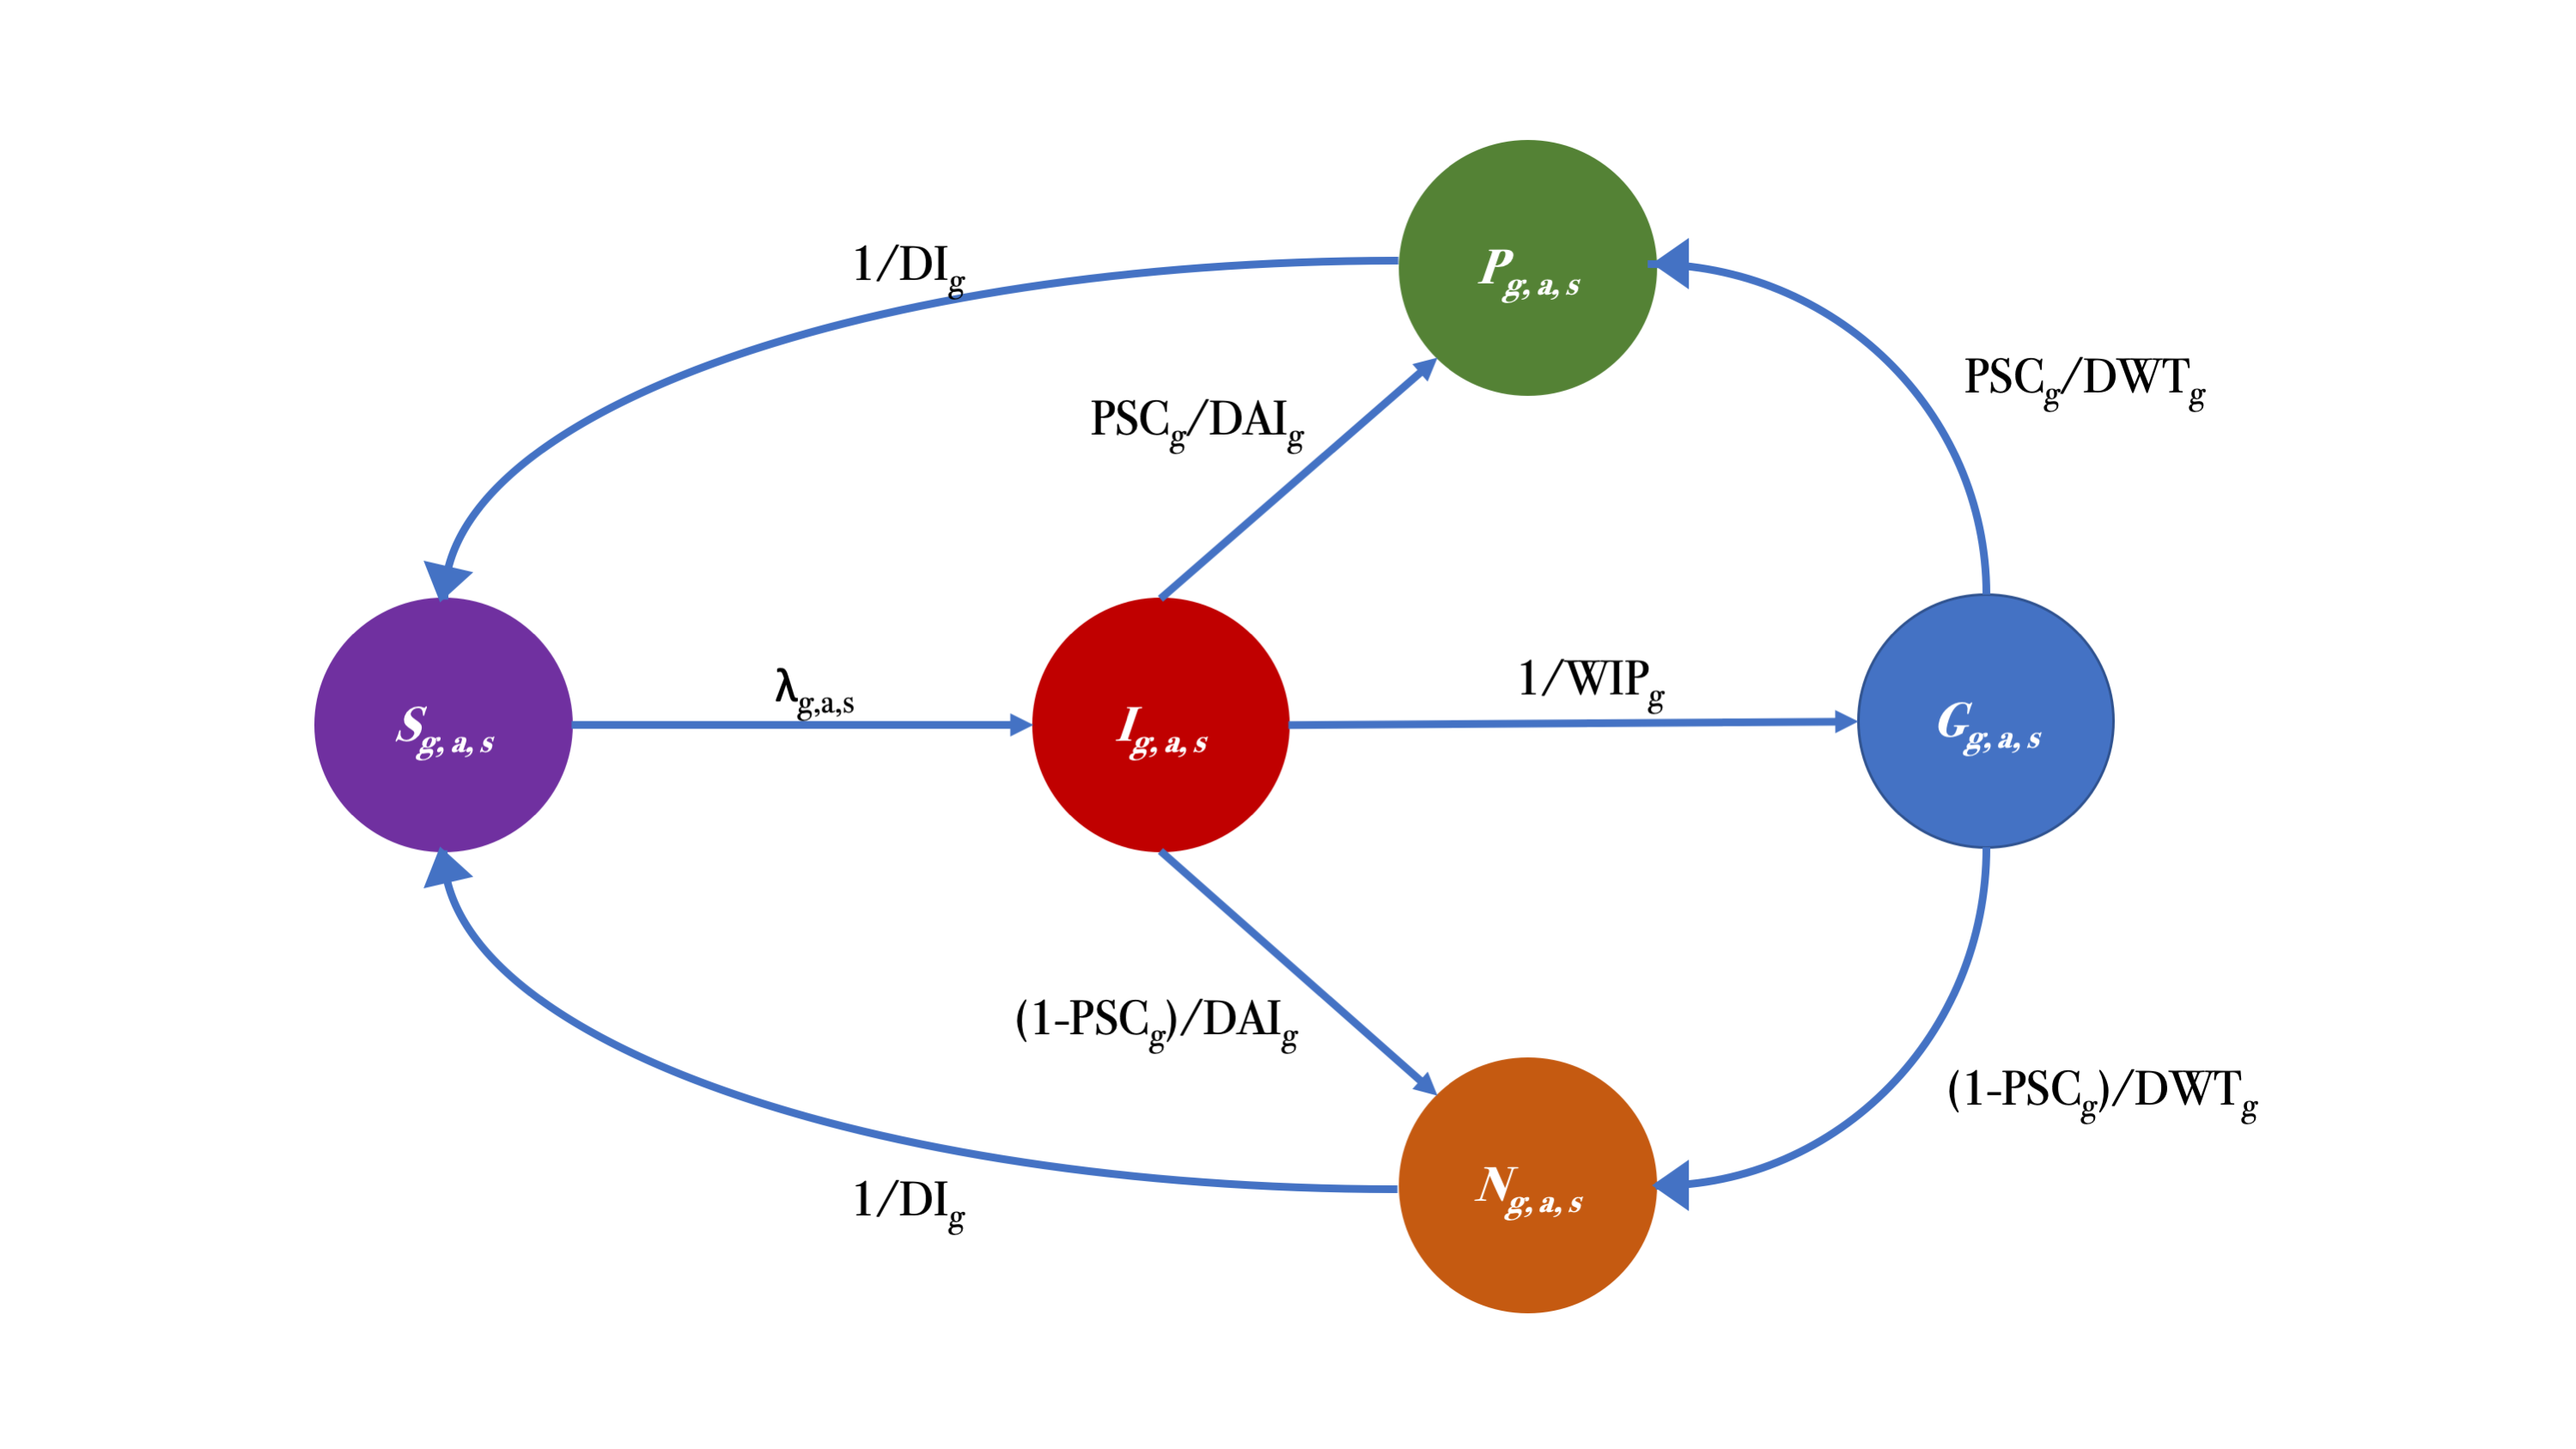
\includegraphics[width=1\textwidth]{COVIDb}
\caption{A compartmental Covid-19 transmission model.}
\label{fig:model}
\end{figure}

The system of ODEs is then formulated as follow

\begin{align*}
\dot{S}_{g,s,a} & =  -\lambda_{g,s,a}(t)S_{g,s,a} + (P_{g,s,a} + N_{g,s,a})/DI_g + \frac{1}{r}S_{g,s,a-1} - \frac{1}{r}S_{g,s,a} + \\
& \quad \frac{1}{R}\sum_{g,s}(S_{g,s,20} + I_{g,s,20} + G_{g,s,20} + P_{g,s,20} + N_{g,s,20}) \times \\
& \quad \delta_1(a)(\pi_1\delta_1(s) + \pi_2\delta_2(s) + \pi_3\delta_3(s) + \pi_4\delta_4(s)) \\ 
\dot{I}_{g,s,a}  & =  \lambda_{g,s,a}(t)S_{g,s,a} - (1/WIP_g + 1/DAI_g)I_{g,s,a} + \frac{1}{r}I_{g,s,a-1}-\frac{1}{r}I_{g,s,a} \\
\dot{G}_{g,s,a}  & =  I_{g,s,a}/WIP_g - G_{g,s,a}/DWT_g + \frac{1}{r}G_{g,s,a-1} - \frac{1}{r}G_{g,s,a} \\ 
\dot{P}_{g,s,a}  & =  PSC_g(I_{g,s,a}/DAI_g + G_{g,s,a}/DWT_g) - P_{g,s,a}/DI_g + \frac{1}{r}P_{g,s,a-1} - \frac{1}{r}P_{g,s,a} \\
\dot{N}_{g,s,a}  & =  (1-PSC_g)(I_{g,s,a}/DAI_g + G_{g,s,a}/DWT_g) - N_{g,s,a}/DI_g + \frac{1}{r}N_{g,s,a-1}-\frac{1}{r}N_{g,s,a} \\
\label{eq:ODE}
\end{align*}

From the Figure \ref{fig:model}, the surveyed population is divided into the following non-overlapping compartments: $S$ is for individuals who are at risk of Covid-19 infection, $I$ is for infected individuals, $G$ is for infected who developed serious symptoms and required ICU admission, $P$ is for those who have recovered, and are seropositive and immune, $N$ is for individuals who are recovered, immune but seronegative. The indices $g$, $a$ and $s$ indicate that every compartment is stratified by gender, age and level of social activity. Movements between compartments are occurring at per capita rates specified by the following parameters: \textbf{PSC} is the probability of becoming seropositive, \textbf{WIP} is the Covid-19 incubation period, \textbf{DAI} is the duration of asymptomatic (i.e. without Covid-19) infection symptoms, \textbf{DWT} is the duration of treatment for Covid-19, and \textbf{DI} is the duration of immunity. Subscripts denote stratification of parameters: for example, \textbf{DWT}$_{g}$ means that in our model this parameter is gender-dependent. Finally, $\lambda$ is the \textbf{force of infection} dependent on the proportion of individuals in $I$ and is defined as

\begin{equation}
\lambda_{g,s,a}=\beta_{g}\sum_{s^{'}, \alpha^{'}} \bigg\{ c^{*}_{g,s,s^{'},\alpha,\alpha^{'}} \frac{I_{g^{'}, s^{'}, \alpha{'}}}{S_{g^{'}, s^{'}, \alpha{'}} + I_{g^{'}, s^{'}, \alpha{'}} + G_{g^{'}, s^{'}, \alpha{'}} + P_{g^{'}, s^{'}, \alpha{'}} + N_{g^{'}, s^{'}, \alpha{'}} } \bigg\}
\end{equation}

with $\beta$ the probability of infection between individuals of different gender. 

\subsection{Model Inputs}

Let $X$ be a time dependent vector that includes the 5 states of the compartmental model, with $X_{g,s,a}(t)=[S_{g,s,a}(t), I_{g,s,a}(t), G_{g,s,a}(t), P_{g,s,a}(t), N_{g,s,a}(t)]$ and $t \in \{1,2,\dots,T \}$. Also, assume that the observations of the model for time $t$ are $O_{g,s,a}(t)=[D_{g,s,a}(t), Y_{g,s,a}(t)]$, with $D_{g,s,a}(t)$ the number of infected and $Y_{g,s,a}(t)$ represents the seroprevalence.

\subsection{Priors}

Next step, after they constructed the compartmental model, was to work on a Bayesian modelling framework that will involve the treatment the parameters of the non-linear system of ODE equations describing the epidemic as unknown random variables. In total, \cite{Gareth:2013} model has 14 parameters with their relevant priors (Table \ref{table:priors})

\begin{table}[h!]
\centering
 \begin{tabular}{||l c r||} 
 \hline
 Parameter & Interpretation & Prior \\ [0.5ex] 
 \hline\hline
 Transmission probability (males) & TRm & $\mathcal{U}[B_a, B_b]$ \\ 
 Transmission probability (females) & TRf & $\mathcal{U}[B_a, B_b]$  \\
 Average incubation period (males) & WIPm & $\mathcal{G}a(k_{WIPm}, \theta_{WIPm})$  \\
 Average incubation period (females) & WIPf & $\mathcal{G}a(k_{WIPf}, \theta_{WIPf})$  \\
 Average duration of treatment (males)  & DWTm & $\mathcal{G}a(k_{DWTm}, \theta_{DWTm})$  \\
 Average duration of treatment (females) & DWTf & $\mathcal{G}a(k_{DWTf}, \theta_{DWTf})$  \\
 Average duration of asymptomatic (males) & DAIm & $\mathcal{G}a(k_{DAIm}, \theta_{DAIm})$  \\
 Average duration of asymptomatic (females) & DAIf & $\mathcal{G}a(k_{DAIf}, \theta_{DAIf})$ \\
 Average duration of immunity (males) & DIm & $\mathcal{U}(k_{DIm}, \theta_{DIm})$ \\
 Average duration of immunity (females) & DIf & $\mathcal{U}(k_{DIf}, \theta_{DIf})$  \\
 Probability of seroconversion (males) & PSCm & $\mathcal{B}e(\alpha_{PSCm}, \beta_{PSCm})$ \\
 Probability of seroconversion (females) & PSCf & $\mathcal{B}e(\alpha_{PSCf}, \beta_{PSCf})$ \\
 Observation error for incidence & $\sigma$ & $inv\mathcal{G}a(k_{\sigma}, \theta_{\sigma})$ \\
 Observation error scale for seroprevalence & $A_{Y}$ & $\mathcal{G}a(k_{A_{Y}}, \theta_{A_{Y}})$  \\ [1ex] 
 \hline
 \end{tabular}
 \caption{Non-linear ODE Model Parameter Priors}
\label{table:priors}
\end{table} 

\subsection{Likelihood}

Here, we present the likelihood model that we will use parameters vector $\theta$ includes the parameters in Table \ref{table:priors} and $X$ includes the ODE states in Equation \ref{eq:ODE}. For efficiency, we symbolise the priors in Table \ref{table:priors} as $\theta$. The observed numbers of new diagnoses are assumed to be observed in Gaussian noise. This assumption is reasonable since the counts obtained are very large, so it is suitable to make a continuous distributional assumption. The likelihood model for the observed seroprevalences is assumed to be a beta distribution since it represents observations of proportions given the parameters. 

\begin{align}
\mathcal{L}(priors, X_{g,s,a}(1), \dots, X_{g,s,a}(t); O_{g,s,a}(1), \dots, O_{g,s,a}(t)) &= \\ 
\Pi_{a}\Pi_{s}\Pi_{g}\Pi_{t}p(O_{g,s,a}(t) | X_{g,s,a}(t), priors) & \\
\Pi_{a}\Pi_{s}\Pi_{g}\Pi_{t}\mathcal{N}(D_{g,s,a}(t)| \mu, \sigma)\mathcal{B}e(Y_{g,s,a}(t)|A_{Y}, B_{Y}) & \\
\label{eq:likelihood}
\end{align}

with the normal distribution mean as

\begin{equation}
\mu = \frac{1}{WIP}\times \frac{I}{S + I + G + N + P}\times 1000
\end{equation}

and the beta distribution scale as $A_{Y}$ and shape 

\begin{equation}
B_{Y} = A_{Y}\bigg( \frac{1}{P} - 1 \bigg)
\end{equation}

\subsection{Posterior}

The posterior of a Bayesian model has the form

\begin{equation}
p(\theta|X, y) \propto p(y|X,\theta)p(\theta|X)
\end{equation}

by replacing the likelihood with Equation \ref{eq:likelihood} and the priors ($\theta$) with Table \ref{table:priors}, we solve for

\begin{equation}
p(\theta|X, y) \propto \Pi_{a}\Pi_{s}\Pi_{g}\Pi_{t}\mathcal{N}(D_{g,s,a}(t)| \mu, \sigma)\mathcal{B}e(Y_{g,s,a}(t)|A_{Y}, B_{Y}) \times \Pi_{i=priors}\theta_{i}
\end{equation}

\bibliographystyle{abbrv}
\bibliography{simple}

\end{document}
This is never printed
